%Capítulo 3

\chapter{Calibración clásica}
\label{ch:classicalCalibration}
\lhead{\emph{Calibración clásica}}
%----------------------------------------------------------------------------------------

\section{Calibración clásica}

Como fue introducido previamente, una antena es alimentada por un generador y consta de una RFDN y un panel de elementos 
radiantes. Como puede variar el comportamiento de cada componente, se utiliza la calibración. En particular, este método se 
lo utiliza para poder medir, detectar y corregir el mal funcionamiento de parte de la RFDN, en particular todas las desviaciones
se las atribuyen los módulos de Transmisión/Recepción. A su vez, también se puede detectar si uno de dichos módulos queda 
inhabilitado a causa que cierta parte de la cadena de transmisión/recepción o dicho componente se destruyó.

Como limitación, esta calibración interna no puede medir las partes pasivas del sistema que están fuera del lazo de
calibración interna (por ejemplo los módulos radiantes), ni la ganancia absoluta, debido a la ausencia de un blanco estándar
de calibración \cite{Wang2010}.

En la figura \ref{fig:classic_cal_scheme} se muestra el esquema de calibración, en el cual se observan tres modos de
calibración. Cada uno posee distintos caminos, \textbf{P1} (líneas rojas) caracteriza el camino de transmisión, \textbf{P2}
(línea azul) caracteriza el camino de recepción y \textbf{P3} la electrónica central (CE) junto a los puertos auxiliares de
transmisión/recepción. \textbf{P3} es utilizado para corregir posibles variaciones en los pulsos \textbf{P1} y \textbf{P2}
\cite{Makhoul2012}. Se puede apreciar que, para este esquema en praticular, tanto los elementos radiantes como sus cables de 
interconexión quedan fuera de los lazos de calibración.

\begin{figure}[H]
 \centering
 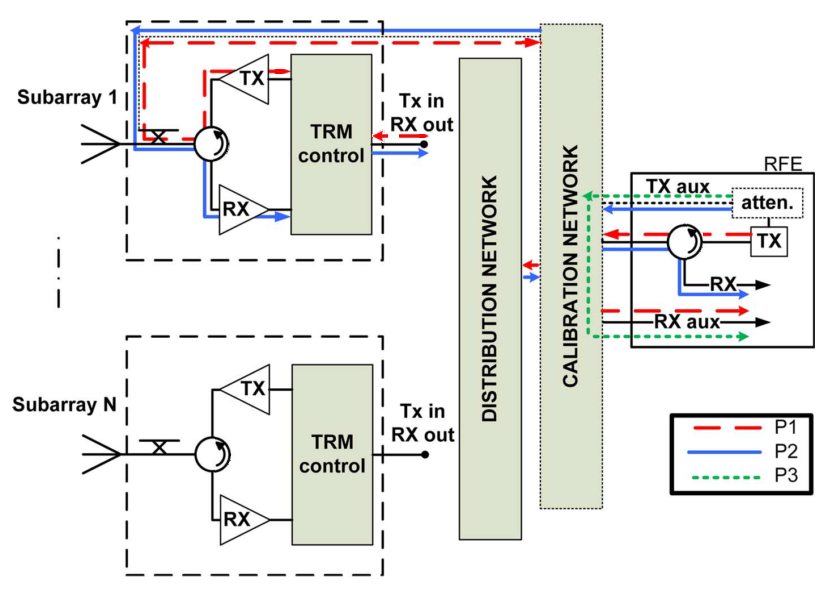
\includegraphics[width=10cm]{gfx/classic_cal_scheme.png}
 \caption{Esquema de calibración interna: camino de calibración de pulsos \textbf{P1} (Tx) en rojo, \textbf{P2} (Rx) en azul
 y \textbf{P3} (electrónica central) en verde \cite{Makhoul2012}.}
 \label{fig:classic_cal_scheme}
\end{figure}

Para dar ejemplos de satélites que utilizaron el método se los puede nombrar al E-ERS-1, el SIR-C \cite{Curlander1991}, el
terraSAR-X \cite{Schwerdt2005}, el ENVISAT ASAR \cite{Loop}, entre otros. La figura \ref{fig:calibrMethods} muestra los esquemas
de calibración de los primeros dos sistemas mencionados.

\begin{figure}[H]
	\centering
	\subfloat[]{
		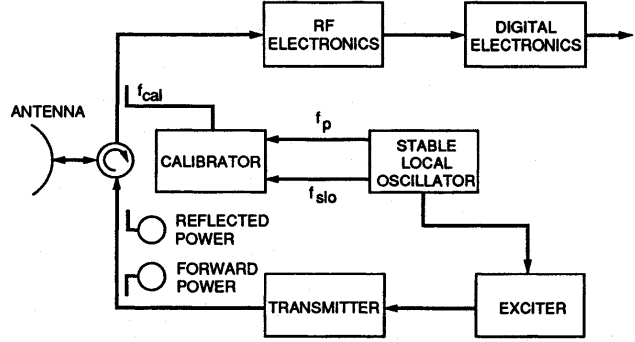
\includegraphics[width=7cm]{gfx/sirCalibration.png}}
 	\subfloat[]{
		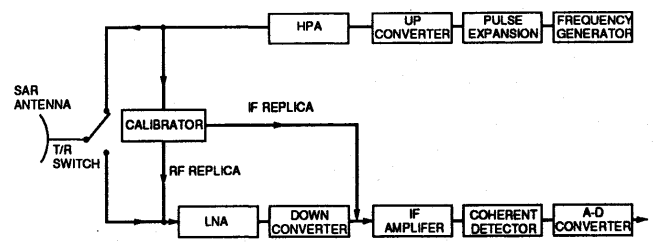
\includegraphics[width=7cm]{gfx/eersCalibration.png}}
	\caption{Esquemas de calibración del SIR-C y E-ERS-1 \cite{Curlander1991}.}
	\label{fig:calibrMethods}
\end{figure}


\subsection{Método} \label{ssc:classicalMethod}

A parte de la medición de la estabilidad del instrumento, es necesario obtener el funcionamiento de los TRMs de forma
individual. Como el apuntamiento y la planitud de la señal dependen de la configuración de estos componentes, es necesario
conocer su estado actual de funcionamiento. Comparando con datos de telemetría (ejemplo temperaturas y tensiones de los
TRMs) junto a apropiada caracterización en tierra solo provee información limitada del comportamiento de la antena \cite{Br2007}.

Una estrategia para mediciones individuales de cada TRM requiere que el resto esté apagado. El problema de esta estrategia
es que, al tener parte de la antena apagada, no resulta un método representativo al modo de funcionamiento nominal (toda la
antena operativa). Para solventar esta problemática y calibrar todos los TRMs a la vez, al menos en transmisión o recepción,
se hace uso de los defasadores para armar un código en que las señales sean ortogonales. En particular, por ejemplo, una de
las usos es defasar cada TRM en $\pm90^{\circ}$ siguiendo una determinada secuencia $c_{mn}(t)$ por cada uno.

\begin{figure}
 \centering
 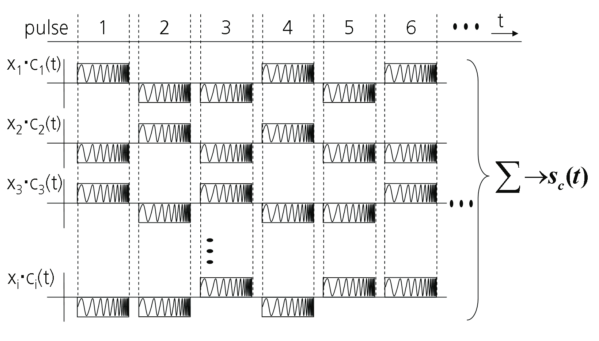
\includegraphics[width=8cm]{gfx/superposition_signals_classic.png}
 \caption{Superposición de señales de todos los TRMs. Cada señal tiene su propia secuencia de código aplicada entre pulsos \cite{Br2007}.}
 \label{fig:sup_sign_classic}
\end{figure}

Por lo tanto, la fase de salida de cada TRM es la fase configurada $\varphi_{mn}$ sumada al defasaje del código de
$90^{\circ}$. Consecuentemente, la superposición de todas las ganancias de los TRMs, $a_{mn}$, y fases, $\varphi_{mn}$,
es obtenida en el puerto de recepción la la RFDN, $s_c(t)$ como se muestra en la figura \ref{fig:sup_sign_classic}.

\begin{equation}
	s_c(t) = \sum_{m=0}^{M-1}\sum_{n=0}^{N-1}c_{mn}\cdot a_{mn}e^{j\varphi{mn}} + n_{mn}
\end{equation}

Donde $n_{mn}$ es el ruido inherente que hay en las mediciones de cada TRM. Para decodificar y obtener la ganancia
$\tilde{a}_{mn}$ y fase estimada $\tilde\varphi_{mn}$ de algún TRM, la señal compuesta $s_c$ es correlacionada con
la secuencia del módulo deseado. Con esta correlación la modulación de la secuencia se elimina dando como resultado
la ganancia estimada.

\begin{equation}
\begin{aligned}
	\tilde{x}_{mn} &= s_c \otimes c^*_{mn} \\
	\tilde{x}_{mn} = \int s_c(t) &\cdot c^*_{mn}(t) dt = \tilde{a}_{mn}e^{j\tilde{\varphi}_{mn}} \\
\end{aligned}
\label{eq:classic_correlation}
\end{equation}

En general el código de calibración utilizado es el código walsh. Dicho código deriva de las matrices de Hadamard (ver
apéndice \ref{AppendixB}); dada sus propiedades de ortogonalidad, cada código, o fila, es unívocamente distinguible del
resto. Para minimizar la cantidad de mediciones, el largo del código ($l$) debe ser lo más corto positble. El número de
TRMs de la antena es el determinante de la cota inferior.

\begin{equation}
	l = 2^i \ge N \cdot M
\end{equation}

Siendo $N$ la cantidad de filas y $M$ la cantidad de paneles, o columnas, que tiene el conjunto de antena. No es necesario que
se calibren todos los TRMs de una. Hay tres estrategias que se utilizan con este método de calibración para obtener
distintos niveles de granularidad de mediciones a saber.

\begin{itemize}
	\item \textbf{Nivel módulo:} Este nivel es el que utiliza los códigos más largos, dado que se calibran todos los módulos que
		posee la antena en una polarización determinada ($l = 2^i \ge N \cdot M$).
	\item \textbf{Nivel panel:} En este nivel se utiliza el mismo código para todos los TRMs que son de un mismo panel,
		logrando así, decrecer el largo del código ($l = 2^i \ge M$).
	\item \textbf{Nivel fila:} En este nivel se utiliza el mismo código para todos los TRMs que son de una misma fila,
		logrando así, decrecer el largo del código ($l = 2^i \ge N$).
\end{itemize}

Este método a nivel panel y fila sirve para la caracterización del la configuración del apuntamiento de antena \cite{Br2007}.

\subsection{Problemas y limitaciones}

La calibración clásica fue diseñada detectar y localizar fallas en los módulos TR permitiendo visualizar como cambia la
fase y atenuación de cada uno a medida que se los comanda a traves de una electrónica central. Como contracara, adolece de
los siguientes problemas:

\begin{itemize}
	\item Caracterización previa de los elementos de antena: Para poder conocer la ganancia del lazo de transmisión o recepción
es necesario conocer la potencia de la señal de calibración, para sustraerla del resultado obtenido. El lazo de calibración
donde se realiza esta medición es el que se muestra en la imagen \ref{fig:classic_cal_scheme}, llamado \textbf{P3}. En esta
medición no se puede determinar cuanto atenúa el lazo, por lo tanto se opta por caracterizar en tierra dichos componentes
para las frecuencias y temperaturas de trabajo.
	\begin{itemize}
		\item Costo de materiales: Comprar materiales que ya vengan caracterizados en temperatura valen el doble que los no
			caracterizados dado que no es un trabajo sencillo y requiere el uso de cámaras de termovacío para realizar los ensayos.
		\item Costo de recursos: La campaña de caracterización puede durar meses, con equipos de trabajo dedicados, lo cual implica
			un gasto de dinero muy importante.
		\item Comportamiento de materiales fin de vida: Como el material envejece, cambia sus propiedades, por lo tanto las mediciones realizadas
			en la campaña de caracterización dejan de tener tanta validez.
	\end{itemize}
	\item Complejidad del hardware de la antena: Como se calibra solo una parte de la antena por vez, transmisión o recepción en
		una u otra polarización (H o V), es necesario que el lazo de calibración esté compuesto por la parte de la antena a
		calibrar junto a hardware dedicado (cables y switches) a esta tarea. Logrando así, no solo que la construcción de la antena
		sea más compleja y que se tengan que caracterizar más componentes, sino también que el defasaje y atenuación que este
		hardware dedicado posee se lo atribuye a los TRMs agregando así más error en la medición.
	\begin{itemize}
		\item Acoplamiento: Como hay hardware agregado, el diseño tiene que se más complicado dado que se incrementan los posibles
			acoplamientos entre componentes.
	\end{itemize}
	\item Inestabilidad del generador: Este método es sumamente susceptible a las variaciones de fase y potencia del generador
		entre pulsos de calibración. Por lo tanto, es de vital importancia armar un generador que sea sumamente estable.
	\item Sistema incompleto: Como hay componentes que están fuera de los lazos de calibración, con el método nunca se puede
		determinar de forma totalmente correcta la ganacia de la antena en cualquiera de sus modos.
	\item A la hora de elegir la longitud del código Walsh, es importante que siempre haya un módulo radiante virtual en la
		antena para evitar la primer columna de la matriz de códigos. En caso contrario el primer TRM siempre tendrá un error en
		la estimación de su ganancia, para mayor información ver \cite{Wang2010}.
	\item Pérdida de ortogonalidad en el código utilizado por comportamiento de defasadores: Si el defasador no tiene un
		comportamiento exactamente igual al configurado a la hora de realizar la calibración, los códigos walsh pierden
		ortogonalidad y, por ende, se logra obtener una mala estimación de los valores de ganancia de la antena.
    \item Compensacion de temperatura en elementos: Se debe mantener la temperatura de los elementos en los valores
        caracterizados para garantizar que las calibraciones sirven.
    \item Es completamente dependiente del modelo y análisis térmico. Por ejemplo, se asume que el comportamiento de los
        módulos radiantes de la antena no varían con la temperatura.
\end{itemize}
